\chapter{Central Forces: Planets and Satellites}\label{ch:b1:central-forces}

Thirty-one satellites circle the Earth twice a day, each one a clock
and a radio, and a phone that hears four of them knows where it is to
a few meters. Halley's comet falls toward the Sun for thirty-eight
years, swings round it in a few weeks, and climbs away again for
thirty-eight more. A probe bound for Mars leaves Earth at exactly the
speed that will make its path just kiss the orbit of Mars. All of this
is the motion of a body attracted toward a fixed point by a force that
falls as the inverse square of the distance, and all of it follows
from two conserved quantities --- energy and \omterm{def:b1:angular-momentum:L}{angular momentum} --- plus
a single new idea, the effective potential. This chapter derives the
orbits' shapes and speeds, Kepler's three laws, and the arithmetic of
putting a satellite where one wants it.

\section{Central conservative forces}

\begin{definition}[Central force; central conservative force]\label{def:b1:central-forces:central}
\index{central force}\index{effective potential energy}
A force is \emph{central} with center $O$ if it is always directed
along $\vect{OM}$: $\vect F = F(M)\,\vect e_r$. It is \emph{central
\omterm{def:b1:work-and-energy:conservative}{conservative}} if its magnitude depends only on $r = OM$: $\vect F =
F(r)\,\vect e_r$, which derives from a \omterm{def:b1:work-and-energy:conservative}{potential energy} $E_p(r)$ with
$F(r) = -\dd E_p/\dd r$.
\end{definition}

\begin{theorem}[Motion under a central conservative force]\label{thm:b1:central-forces:reduction}
\index{law of areas}
A particle of mass $m$ subject only to a \omterm{def:b1:central-forces:central}{central conservative} force:
\begin{enumerate}
  \item keeps its \omterm{def:b1:angular-momentum:L}{angular momentum} $\vect L_O$; its motion is planar and,
        in \omterm{def:b1:point-kinematics:cylindrical}{polar coordinates} in that plane, $r^2\dot\theta = C$ is
        constant (law of areas, \cref{cor:b1:angular-momentum:central});
  \item keeps its \omterm{thm:b1:work-and-energy:em}{mechanical energy} $E_m = \tfrac12 m(\dot r^2 + r^2\dot\theta^2)
        + E_p(r)$, which can be written
        \[
        E_m = \tfrac12 m\dot r^2 + E_{p,\mathrm{eff}}(r), \qquad
        E_{p,\mathrm{eff}}(r) = E_p(r) + \frac{mC^2}{2r^2} = E_p(r) + \frac{L^2}{2mr^2} .
        \]
\end{enumerate}
The radial motion is thus that of a one-dimensional particle in the
\emph{effective potential} $E_{p,\mathrm{eff}}$: the radial \omterm{def:b1:work-and-energy:turning}{turning
points} are the roots of $E_{p,\mathrm{eff}}(r) = E_m$, the motion is
bound if it is trapped between two of them, and circular if $r$ sits at
a minimum of $E_{p,\mathrm{eff}}$.
\end{theorem}

\begin{proof}
Part 1 is \cref{cor:b1:angular-momentum:central}. The force is
\omterm{def:b1:work-and-energy:conservative}{conservative} and no other force acts, so $E_m$ is conserved; in the
plane, $v^2 = \dot r^2 + r^2\dot\theta^2$ and $r^2\dot\theta^2 = C^2/r^2$.
The term $mC^2/2r^2$, the \omterm{thm:b1:work-and-energy:ke}{kinetic energy} of the angular motion, acts as
a repulsive \emph{\omterm{prop:b1:central-forces:effective}{centrifugal barrier}} in the radial problem, to which
the one-dimensional analysis of \cref{ch:b1:work-and-energy} applies.
\end{proof}

\section{Newtonian gravitation}

\begin{definition}[Universal gravitation]\label{def:b1:central-forces:gravitation}
\index{gravitation}\index{gravitational potential energy}
A point mass $M$ at $O$ attracts a point mass $m$ at $M$ with
\[
\vect F = -\frac{GMm}{r^2}\,\vect e_r, \qquad E_p = -\frac{GMm}{r} \quad (E_p \to 0 \text{ at infinity}),
\]
$G = \qty{6.67e-11}{N.m^2/kg^2}$. A spherically symmetric body attracts
outside itself as if its mass were at its center (admitted; a
consequence of Gauss's theorem, \cref{ch:b1:electrostatics-gauss}).
\end{definition}

\begin{proposition}[The effective potential of gravitation]\label{prop:b1:central-forces:effective}
\index{centrifugal barrier}\index{circular orbit}
For $E_p = -GMm/r$,
\[
E_{p,\mathrm{eff}}(r) = -\frac{GMm}{r} + \frac{L^2}{2mr^2}
\]
tends to $+\infty$ at $r \to 0$ (for $L \neq 0$), to $0^-$ at infinity,
and has one minimum at $r_c = L^2/GMm^2$, of value $-G^2M^2m^3/2L^2$.
Hence: $E_m < 0$ --- \omterm{def:b1:work-and-energy:turning}{bound motion} between a minimum and a maximum
radius (perigee and apogee); $E_m \geq 0$ --- unbound, the body comes
from and returns to infinity; $E_m$ equal to the minimum --- \omterm{prop:b1:central-forces:effective}{circular
orbit} of radius $r_c$.
\end{proposition}

\begin{proof}
Limits by inspection; $E_{p,\mathrm{eff}}' = GMm/r^2 - L^2/mr^3 = 0$ at
$r_c$; substitute. The circular case is $\dot r = 0$ forever, possible
only at the minimum.
\end{proof}

\begin{omfigure}
\begin{tikzpicture}
\begin{axis}[omaxis, axis x line=bottom, axis y line=left, width=10.5cm, height=6cm, xlabel={$r/r_c$}, ylabel={$E_{p,\mathrm{eff}}$},
    xlabel style={at={(axis description cs:0.5,-0.06)}, anchor=north},
    xmin=0, xmax=6, ymin=-1.2, ymax=1.2, xtick={1,2,3,4,5}, ytick={-1,0,1}, yticklabels={$-\frac{GMm}{2r_c}$,$0$,}]
  \addplot[omDef, thick, domain=0.36:6, samples=300] {-2/x + 1/x^2};
  \addplot[omExo, dashed, domain=0:6, samples=2] {0};
  \addplot[omThm, dashed, domain=0:6, samples=2] {-0.5};
  \addplot[omProp, dashed, domain=0:6, samples=2] {0.4};
  \draw[Stealth-Stealth, omThm] (axis cs:0.586,-0.5) -- (axis cs:3.41,-0.5);
  \node[omThm, font=\footnotesize, above] at (axis cs:2.0,-0.48) {$E_m < 0$: ellipse};
  \node[omProp, font=\footnotesize, above] at (axis cs:3.5,0.42) {$E_m > 0$: hyperbola};
  \node[omExo, font=\footnotesize, above] at (axis cs:4.8,0.02) {$E_m = 0$: parabola};
  \fill[omDef] (axis cs:1,-1) circle (1.5pt); \node[omDef, font=\footnotesize, right] at (axis cs:1.15,-1.0) {circular};
  \node[font=\footnotesize, omDef] at (axis cs:0.9,0.8) {$\dfrac{L^2}{2mr^2}$};
  \node[font=\footnotesize, omDef] at (axis cs:5.2,-0.72) {$-\dfrac{GMm}{r}$};
\end{axis}
\end{tikzpicture}

{\small The effective potential of Newtonian \omterm{def:b1:central-forces:gravitation}{gravitation}: the
attraction $-GMm/r$ plus the \omterm{prop:b1:central-forces:effective}{centrifugal barrier} $L^2/2mr^2$. Below
zero energy the radial motion is trapped between two \omterm{def:b1:work-and-energy:turning}{turning points}
(perigee, apogee); at the minimum the orbit is circular; at or above
zero the body escapes.}
\end{omfigure}

\begin{theorem}[Circular orbits]\label{thm:b1:central-forces:circular}
\index{orbital speed}\index{Kepler's third law}
On a \omterm{prop:b1:central-forces:effective}{circular orbit} of radius $r$ about a mass $M$:
\[
v = \sqrt{\frac{GM}{r}}, \qquad
T = 2\pi\sqrt{\frac{r^3}{GM}}, \qquad
E_m = -\frac{GMm}{2r} = -E_k = \tfrac12 E_p .
\]
In particular $T^2/r^3 = 4\pi^2/GM$ is the same for all \omterm{prop:b1:central-forces:effective}{circular orbits}
about the same center (\omterm{thm:b1:central-forces:circular}{Kepler's third law}).
\end{theorem}

\begin{proof}
Uniform \omterm{cor:b1:point-kinematics:circular}{circular motion} needs the \omterm{prop:b1:newton-dynamics:centripetal}{centripetal force} $mv^2/r = GMm/r^2$;
$T = 2\pi r/v$; $E_k = \tfrac12 mv^2 = GMm/2r$ and $E_p = -GMm/r$.
\end{proof}

\begin{example}[Three orbits]\label{ex:b1:central-forces:orbits}
$GM_\oplus = \qty{3.99e14}{m^3/s^2}$. Low orbit ($r = \qty{6770}{km}$,
\qty{400}{km} up): $v = \qty{7.7}{km/s}$, $T = \qty{92}{min}$. Geostationary
($T = \qty{86164}{s}$, one sidereal day): $r = (GMT^2/4\pi^2)^{1/3} =
\qty{42200}{km}$, $v = \qty{3.1}{km/s}$. The Moon ($r = \qty{384000}{km}$):
$T = \qty{27.4}{d}$ --- and its \omterm{cor:b1:point-kinematics:circular}{centripetal acceleration} $v^2/r =
\qty{2.7e-3}{m/s^2}$ is $g/3600$ at sixty Earth radii: the inverse
square, checked by Newton himself.
\end{example}

\section{Kepler's laws and the shape of orbits}

\begin{theorem}[Trajectories in a Newtonian field]\label{thm:b1:central-forces:conics}
\index{Kepler's laws}\index{conic}\index{ellipse (orbit)}\index{eccentricity}
The \omterm{def:b1:point-kinematics:frame}{trajectory} of a body in the field of a fixed mass $M$ is a conic
with $O$ at one focus: an ellipse if $E_m < 0$, a parabola if $E_m = 0$,
a hyperbola if $E_m > 0$. For the ellipse of semi-major axis $a$ and
eccentricity $e$:
\begin{itemize}
  \item (Kepler I) the center of force is at a focus; perigee and apogee
        are at $r_p = a(1 - e)$ and $r_a = a(1 + e)$;
  \item (Kepler II) the \omterm{cor:b1:angular-momentum:central}{areal velocity} is constant (the law of areas);
  \item (Kepler III) the period obeys $T^2 = 4\pi^2a^3/GM$;
  \item the energy depends on $a$ alone, $E_m = -GMm/2a$, so that the
        speed at distance $r$ is given by
        \[
        v^2 = GM\left(\frac{2}{r} - \frac{1}{a}\right) .
        \]
\end{itemize}
\end{theorem}
\admitted

\begin{remark}[What is proved and what is admitted]\label{rem:b1:central-forces:admitted}
Kepler II and the energy classification were proved above. That the
bound orbits are exactly ellipses with $O$ at a focus, with Kepler III
and $E_m = -GMm/2a$ in general, needs the integration of the radial
equation (the Year 2 volume does it); for \omterm{prop:b1:central-forces:effective}{circular orbits} ($a = r$,
$e = 0$) every statement reduces to \cref{thm:b1:central-forces:circular},
which is the check we can make here. The relation $v^2 = GM(2/r - 1/a)$
follows from $E_m = \tfrac12 mv^2 - GMm/r = -GMm/2a$ once that energy
formula is granted.
\end{remark}

\begin{omfigure}
\begin{tikzpicture}[font=\small, x=1cm, y=1cm]
  % ellipse a=3, e=0.6, c=1.8, b=2.4 ; focus O at origin ; center at (-1.8,0)
  \draw[omDef, thick] (-1.8,0) ellipse (3 and 2.4);
  \fill (0,0) circle (1.8pt) node[below] {$O$};
  \fill (-3.6,0) circle (1.2pt) node[below] {$O'$};
  \draw[dashed] (-4.8,0) -- (1.2,0);
  \fill[omThm] (1.2,0) circle (1.6pt) node[below right] {$P$};
  \fill[omThm] (-4.8,0) circle (1.6pt) node[below left] {$A$};
  \draw[Stealth-Stealth, omExo] (-1.8,-2.6) -- (1.2,-2.6) node[midway, below] {$a$};
  \draw[Stealth-Stealth, omExo] (-1.8,0.1) -- (-1.8,2.4) node[midway, left] {$b$};
  \draw[Stealth-Stealth, omExo] (-1.8,0.45) -- (0,0.45) node[midway, above] {$c = ea$};
  \node[omThm, font=\footnotesize] at (0.7,0.8) {$r_p = a(1 - e)$};
  \node[omThm, font=\footnotesize] at (-3.4,0.8) {$r_a = a(1 + e)$};
  % hyperbola and parabola sketches on the right
  \begin{scope}[xshift=6.3cm]
  \fill (0,0) circle (1.8pt) node[below] {$O$};
  \draw[omProp, thick, domain=-1.55:1.55, samples=80, variable=\t] plot ({1.0*cosh(\t)-1.6},{1.2*sinh(\t)});
  \draw[omExo, thick, domain=-2.4:2.4, samples=80, variable=\y] plot ({0.5*\y*\y-2.6},{\y});
  \node[omProp, font=\footnotesize] at (0.0,2.9) {$E_m > 0$};
  \node[omExo, font=\footnotesize] at (-2.2,2.9) {$E_m = 0$};
  \end{scope}
\end{tikzpicture}

{\small Left: an elliptical orbit about the focus $O$ --- semi-major
axis $a$, semi-minor $b$, focal distance $c = ea$; the body is fastest at
the perigee $P$ and slowest at the apogee $A$. Right: a hyperbola (positive
energy) and a parabola (zero energy) about the same focus --- the unbound
paths of comets and probes.}
\end{omfigure}

\begin{example}[Halley's comet]\label{ex:b1:central-forces:halley}
Perihelion \qty{0.586}{AU}, aphelion \qty{35.1}{AU}: $a = \qty{17.8}{AU}$,
$e = 0.967$, $T = \sqrt{17.8^3} = \qty{75}{years}$ (Kepler III in
astronomical units and years, where $T^2 = a^3$ for the Sun). With
$GM_\odot = \qty{1.33e20}{m^3/s^2}$, the speed at perihelion is
$\sqrt{GM(2/r_p - 1/a)} = \qty{54}{km/s}$ and at aphelion \qty{0.9}{km/s}
--- sixty times slower, as the law of areas demands ($r_pv_p = r_av_a$).
\end{example}

\section{Satellites}

\begin{proposition}[Escape velocity; geostationary orbit]\label{prop:b1:central-forces:escape}
\index{escape velocity}\index{geostationary orbit}
From the surface of a body of mass $M$ and radius $R$, the minimum
launch speed to reach infinity is $v_e = \sqrt{2GM/R} = \sqrt2\,v_c$,
where $v_c = \sqrt{GM/R}$ is the circular speed at ground level:
\qty{11.2}{km/s} for the Earth. A \emph{geostationary} satellite orbits
in the equatorial plane with the Earth's sidereal period, at
$r = \qty{42200}{km}$ (\qty{35800}{km} above ground).
\end{proposition}

\begin{proof}
$E_m \geq 0$: $\tfrac12 mv_e^2 - GMm/R = 0$. Kepler III with $T = \qty{86164}{s}$.
\end{proof}

\begin{proposition}[Hohmann transfer]\label{prop:b1:central-forces:hohmann}
\index{Hohmann transfer}
To move a satellite from a \omterm{prop:b1:central-forces:effective}{circular orbit} of radius $r_1$ to a coplanar
\omterm{prop:b1:central-forces:effective}{circular orbit} of radius $r_2 > r_1$ with two brief burns, fire at $r_1$
to enter the \emph{transfer ellipse} of perigee $r_1$ and apogee $r_2$
($a = (r_1 + r_2)/2$), coast half a period, and fire again at $r_2$ to
circularize:
\[
\Delta v_1 = \sqrt{\frac{GM}{r_1}}\left(\sqrt{\frac{2r_2}{r_1 + r_2}} - 1\right),
\qquad
\Delta v_2 = \sqrt{\frac{GM}{r_2}}\left(1 - \sqrt{\frac{2r_1}{r_1 + r_2}}\right),
\qquad
t = \pi\sqrt{\frac{(r_1 + r_2)^3}{8GM}} .
\]
\end{proposition}

\begin{proof}
Speeds on the transfer ellipse from $v^2 = GM(2/r - 1/a)$ at $r_1$ and
$r_2$; subtract the circular speeds; half the period of
\cref{thm:b1:central-forces:conics}.
\end{proof}

\begin{omfigure}
\begin{tikzpicture}[font=\small, x=1cm, y=1cm]
  \fill (0,0) circle (2.5pt) node[below left] {$O$};
  \draw[omDef, thick] (0,0) circle (1.0);
  \draw[omDef, thick] (0,0) circle (3.0);
  % transfer ellipse: perigee r1=1 at (1,0), apogee r2=3 at (-3,0): a=2, c=1, center (-1,0), b=sqrt(3)=1.732
  \draw[omThm, thick] (-1,0) ellipse (2 and 1.732);
  \fill[omThm] (1,0) circle (1.6pt); \fill[omThm] (-3,0) circle (1.6pt);
  \draw[-Stealth, omExo, very thick] (1,0) -- (1,1.0) node[right] {$\Delta v_1$};
  \draw[-Stealth, omExo, very thick] (-3,0) -- (-3,-0.8) node[left] {$\Delta v_2$};
  \node[omDef, font=\footnotesize] at (1.5,-1.2) {$r_1$};
  \node[omDef, font=\footnotesize] at (2.6,2.3) {$r_2$};
  \node[omThm, font=\footnotesize] at (-1.0,2.0) {transfer ellipse};
  \draw[-Stealth, omThm] (-0.2,1.72) -- (-0.8,1.73);
\end{tikzpicture}

{\small A \omterm{prop:b1:central-forces:hohmann}{Hohmann transfer} between two \omterm{prop:b1:central-forces:effective}{circular orbits}: a first burn at
the inner orbit raises the apogee to $r_2$; half an ellipse later a
second burn raises the perigee --- the least-fuel two-burn route, and
the one that takes a probe to Mars.}
\end{omfigure}

\begin{example}[Low orbit to geostationary]\label{ex:b1:central-forces:leogeo}
$r_1 = \qty{6770}{km}$, $r_2 = \qty{42200}{km}$: $\Delta v_1 = \qty{2.4}{km/s}$,
$\Delta v_2 = \qty{1.5}{km/s}$, coast \qty{5.3}{h}. The total,
\qty{3.9}{km/s}, is half what the launch to low orbit already cost: the
``last mile'' to a high orbit is expensive, and satellites carry their own
engine for it.
\end{example}

\begin{remark}[Repulsive centers]\label{rem:b1:central-forces:rutherford}
\index{Rutherford scattering}
For a repulsive inverse-square force (two like charges,
\cref{ch:b1:electrostatics-gauss}) the effective potential has no well:
every \omterm{def:b1:point-kinematics:frame}{trajectory} is a hyperbola, the particle approaches, is deflected
and leaves. Aiming an $\alpha$ particle straight at a gold nucleus, its
distance of closest approach follows from energy alone, $E_k =
2Ze^2/4\pi\varepsilon_0 r_{\min}$ --- Rutherford's way of bounding the size of
the nucleus (\cref{exo:b1:central-forces:11}).
\end{remark}

\section{Exercises}

\begin{exercise}[$\star$]\label{exo:b1:central-forces:1}
The International Space Station orbits at \qty{400}{km} altitude
($R_\oplus = \qty{6370}{km}$, $GM_\oplus = \qty{3.99e14}{m^3/s^2}$). Speed,
period, number of sunrises its crew sees per day.
\end{exercise}

\begin{exercise}[$\star$]\label{exo:b1:central-forces:2}
Find the radius and altitude of the \omterm{prop:b1:central-forces:escape}{geostationary orbit} from the
sidereal day \qty{86164}{s}, and the \omterm{thm:b1:central-forces:circular}{orbital speed}.
\end{exercise}

\begin{exercise}[$\star$]\label{exo:b1:central-forces:3}
\omterm{prop:b1:central-forces:escape}{Escape velocity} from the Earth and from the Moon ($GM = \qty{4.90e12}{m^3/s^2}$,
$R = \qty{1740}{km}$). Why does the Moon keep no atmosphere?
\end{exercise}

\begin{exercise}[$\star$]\label{exo:b1:central-forces:4}
Mars has $a = \qty{1.524}{AU}$, Jupiter \qty{5.20}{AU}: their years, from
\omterm{thm:b1:central-forces:circular}{Kepler's third law}. A body at \qty{30}{AU} (Neptune)?
\end{exercise}

\begin{exercise}[$\star\star$]\label{exo:b1:central-forces:5}
Energy needed to place \qty{1000}{kg} on the ISS orbit starting from
rest at the surface (ignore the Earth's rotation and the air). Compare
with the chemical energy of gasoline (\qty{46}{MJ/kg}).
\end{exercise}

\begin{exercise}[$\star\star$]\label{exo:b1:central-forces:6}
Halley's comet: perihelion \qty{0.586}{AU}, aphelion \qty{35.1}{AU}.
Compute $a$, $e$, the period, and the speeds at perihelion and aphelion
($GM_\odot = \qty{1.33e20}{m^3/s^2}$, $\qty{1}{AU} = \qty{1.496e11}{m}$).
\end{exercise}

\begin{exercise}[$\star\star$]\label{exo:b1:central-forces:7}
\omterm{prop:b1:central-forces:hohmann}{Hohmann transfer} from the ISS orbit (\qty{6770}{km}) to the
\omterm{prop:b1:central-forces:escape}{geostationary orbit} (\qty{42200}{km}): both burns, total, and duration.
\end{exercise}

\begin{exercise}[$\star\star$]\label{exo:b1:central-forces:8}
Show that the minimum of $E_{p,\mathrm{eff}}$ sits at $r_c = L^2/GMm^2$,
and that small radial oscillations about it have the \omterm{def:b1:wave-propagation:signal}{angular frequency}
$\sqrt{GM/r_c^3}$ --- the orbital frequency itself. What does this say
about a slightly disturbed \omterm{prop:b1:central-forces:effective}{circular orbit}?
\end{exercise}

\begin{exercise}[$\star\star$]\label{exo:b1:central-forces:9}
Astronauts aboard the ISS float. Explain with the forces; what is the
value of $g$ at their altitude, and why does it not contradict the
floating?
\end{exercise}

\begin{exercise}[$\star\star\star$]\label{exo:b1:central-forces:10}
Newton's ``Moon test'': compute the Moon's \omterm{cor:b1:point-kinematics:circular}{centripetal acceleration} from
$r = \qty{3.84e8}{m}$ and $T = \qty{27.3}{d}$, and compare with
$g(R/r)^2$. Conclude.
\end{exercise}

\begin{exercise}[$\star\star\star$]\label{exo:b1:central-forces:11}
An $\alpha$ particle ($q = 2e$, $E_k = \qty{5.0}{MeV}$) is fired straight
at a gold nucleus ($Z = 79$), taken fixed. Using energy conservation
with $E_p = 2Ze^2/4\pi\varepsilon_0r$ ($1/4\pi\varepsilon_0 = \qty{8.99e9}{SI}$),
find the distance of closest approach; compare with the nuclear radius,
about \qty{7}{fm}. What energy would be needed to touch the nucleus?
\end{exercise}

\begin{exercise}[$\star\star\star$]\label{exo:b1:central-forces:12}
A satellite in low orbit is slowed by the residual atmosphere, so its
\omterm{thm:b1:work-and-energy:em}{mechanical energy} decreases. Show with $E_m = -GMm/2r$ and
$v = \sqrt{GM/r}$ that it then moves \emph{faster}. Where does the
energy go, and what fraction of the lost \omterm{def:b1:work-and-energy:conservative}{potential energy} becomes heat?
\end{exercise}

\begin{omfigure}
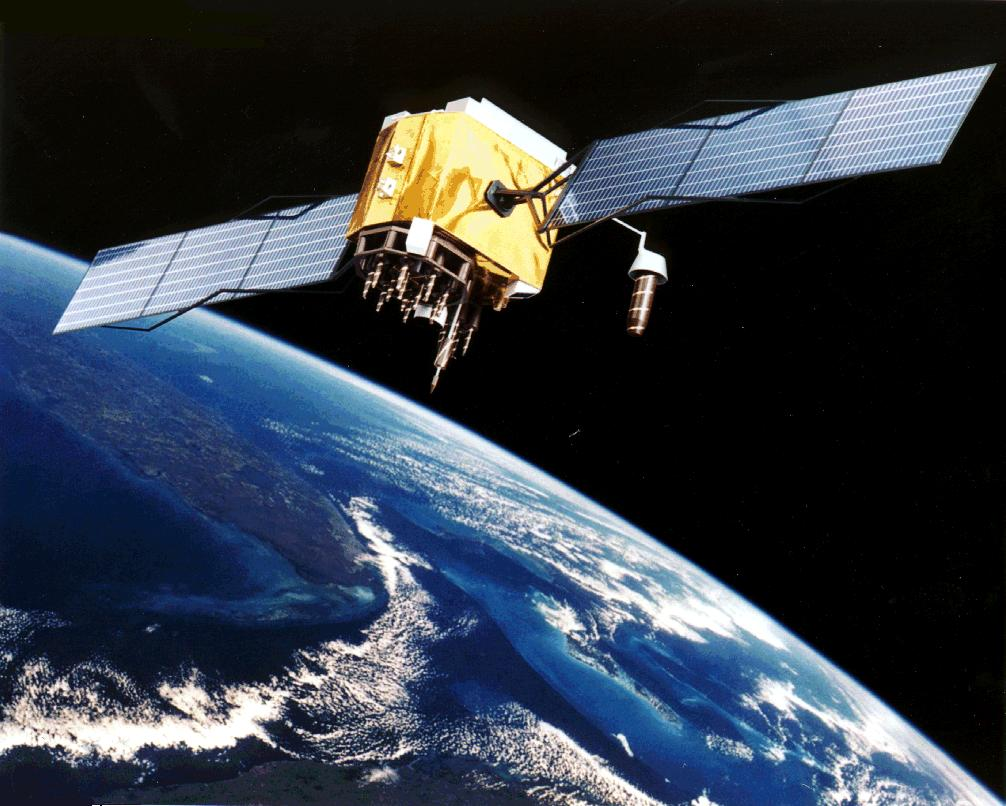
\includegraphics[width=0.46\linewidth]{images/book3/gps-satellite-nasa.jpg}

{\small A GPS satellite (NASA artist's view): one of the thirty-odd in the \qty{20200}{km} constellation of the weekend problem, each a clock in a Keplerian orbit.}
\end{omfigure}

\section{Problem: The satellites that tell you where you are}

\begin{problem}[{Weekend problem --- a navigation constellation twenty
thousand kilometers up: its orbit, the fuel to get there, how many
satellites a phone can see, and why their clocks must be told to run
slow}]
\label{pb:b1:central-forces:1}
Data: $GM_\oplus = \qty{3.986e14}{m^3/s^2}$, $R_\oplus = \qty{6371}{km}$,
sidereal day \qty{86164}{s}, $c = \qty{2.998e8}{m/s}$. The satellites
circle the Earth in exactly half a sidereal day on \omterm{prop:b1:central-forces:effective}{circular orbits}.

\medskip
\noindent\textbf{Part I --- The orbit.}
\begin{enumerate}
  \item Compute the orbital radius and the altitude.
  \item Compute the \omterm{thm:b1:central-forces:circular}{orbital speed}.
  \item Compute the satellite's acceleration and compare it with $g$ at
        the surface.
  \item Compute the \omterm{thm:b1:work-and-energy:em}{mechanical energy} per kilogram, and the kinetic and
        potential parts.
  \item Why choose half a sidereal day rather than half a solar day?
        What does a ground observer see repeat?
  \item Seen from a satellite, what angle does the Earth's disk subtend?
  \item Compare the orbit's radius with the geostationary one; which is
        higher, and by what factor?
\end{enumerate}

\medskip
\noindent\textbf{Part II --- Getting there.}
\begin{enumerate}[resume]
  \item Energy per kilogram to go from rest at the surface to the final
        orbit (ignore the air and the Earth's spin).
  \item The launcher first reaches a low \omterm{prop:b1:central-forces:effective}{circular orbit} at \qty{400}{km}.
        Speed there?
  \item \omterm{prop:b1:central-forces:hohmann}{Hohmann transfer} from that orbit to the final one: the two burns
        and their sum.
  \item Duration of the transfer.
  \item Compare the sum of the burns with the \omterm{prop:b1:central-forces:escape}{escape velocity} from low
        orbit: how far from ``leaving the Earth'' is this mission?
  \item The upper stage and satellite mass \qty{2000}{kg} before the
        transfer; the engine's exhaust speed is \qty{3.0}{km/s} and the
        rocket equation gives $\Delta v = u\ln(m_0/m_1)$. Propellant
        needed for the two burns?
\end{enumerate}

\medskip
\noindent\textbf{Part III --- Coverage and timing.}
\begin{enumerate}[resume]
  \item A satellite is visible from every point of the Earth that lies
        within the cone of half-angle $\theta$ with $\cos\theta = R/r$
        about the Earth--satellite line. Compute $\theta$ and the
        fraction $(1 - \cos\theta)/2$ of the Earth's surface it covers.
  \item With $24$ satellites spread uniformly, how many are visible on
        average from one point? Is the minimum of $4$ needed for a fix
        plausible?
  \item Light travel time from a satellite at the zenith; at the
        horizon.
  \item To locate the receiver to \qty{3}{m}, to what precision must the
        \omterm{def:b1:wave-propagation:signal}{signals} be timed?
  \item The receiver's own clock is a cheap quartz, wrong by
        milliseconds: why are four satellites needed instead of three?
  \item The satellites' clocks are atomic. Give the relative stability
        needed for a \qty{3}{m} error after one day.
\end{enumerate}

\medskip
\noindent\textbf{Part IV --- Relativity, briefly.}
Two effects shift the satellite clocks relative to ground clocks
(formulas admitted, from the Year 3 volume): motion slows a clock by the
fraction $v^2/2c^2$; height speeds it up by $GM(1/R - 1/r)/c^2$.
\begin{enumerate}[resume]
  \item Compute the slowing due to speed, in microseconds per day.
  \item Compute the speeding-up due to altitude, in microseconds per
        day.
  \item Net effect, and the position error it would cause per day if
        uncorrected.
  \item The satellite clocks are set before launch to
        \qty{10.22999999543}{MHz} instead of \qty{10.23}{MHz}. Check that
        this compensates the net effect.
  \item The orbits are not exactly Keplerian: name three perturbations
        and say how the system copes.
  \item Summarize the chain: two conservation laws, one orbit, one
        constellation, and the one correction nobody would have guessed.
\end{enumerate}
\end{problem}
